% Options for packages loaded elsewhere
\PassOptionsToPackage{unicode}{hyperref}
\PassOptionsToPackage{hyphens}{url}
%
\documentclass[
]{article}
\usepackage{amsmath,amssymb}
\usepackage{iftex}
\ifPDFTeX
  \usepackage[T1]{fontenc}
  \usepackage[utf8]{inputenc}
  \usepackage{textcomp} % provide euro and other symbols
\else % if luatex or xetex
  \usepackage{unicode-math} % this also loads fontspec
  \defaultfontfeatures{Scale=MatchLowercase}
  \defaultfontfeatures[\rmfamily]{Ligatures=TeX,Scale=1}
\fi
\usepackage{lmodern}
\ifPDFTeX\else
  % xetex/luatex font selection
\fi
% Use upquote if available, for straight quotes in verbatim environments
\IfFileExists{upquote.sty}{\usepackage{upquote}}{}
\IfFileExists{microtype.sty}{% use microtype if available
  \usepackage[]{microtype}
  \UseMicrotypeSet[protrusion]{basicmath} % disable protrusion for tt fonts
}{}
\makeatletter
\@ifundefined{KOMAClassName}{% if non-KOMA class
  \IfFileExists{parskip.sty}{%
    \usepackage{parskip}
  }{% else
    \setlength{\parindent}{0pt}
    \setlength{\parskip}{6pt plus 2pt minus 1pt}}
}{% if KOMA class
  \KOMAoptions{parskip=half}}
\makeatother
\usepackage{xcolor}
\usepackage[margin=1in]{geometry}
\usepackage{color}
\usepackage{fancyvrb}
\newcommand{\VerbBar}{|}
\newcommand{\VERB}{\Verb[commandchars=\\\{\}]}
\DefineVerbatimEnvironment{Highlighting}{Verbatim}{commandchars=\\\{\}}
% Add ',fontsize=\small' for more characters per line
\usepackage{framed}
\definecolor{shadecolor}{RGB}{248,248,248}
\newenvironment{Shaded}{\begin{snugshade}}{\end{snugshade}}
\newcommand{\AlertTok}[1]{\textcolor[rgb]{0.94,0.16,0.16}{#1}}
\newcommand{\AnnotationTok}[1]{\textcolor[rgb]{0.56,0.35,0.01}{\textbf{\textit{#1}}}}
\newcommand{\AttributeTok}[1]{\textcolor[rgb]{0.13,0.29,0.53}{#1}}
\newcommand{\BaseNTok}[1]{\textcolor[rgb]{0.00,0.00,0.81}{#1}}
\newcommand{\BuiltInTok}[1]{#1}
\newcommand{\CharTok}[1]{\textcolor[rgb]{0.31,0.60,0.02}{#1}}
\newcommand{\CommentTok}[1]{\textcolor[rgb]{0.56,0.35,0.01}{\textit{#1}}}
\newcommand{\CommentVarTok}[1]{\textcolor[rgb]{0.56,0.35,0.01}{\textbf{\textit{#1}}}}
\newcommand{\ConstantTok}[1]{\textcolor[rgb]{0.56,0.35,0.01}{#1}}
\newcommand{\ControlFlowTok}[1]{\textcolor[rgb]{0.13,0.29,0.53}{\textbf{#1}}}
\newcommand{\DataTypeTok}[1]{\textcolor[rgb]{0.13,0.29,0.53}{#1}}
\newcommand{\DecValTok}[1]{\textcolor[rgb]{0.00,0.00,0.81}{#1}}
\newcommand{\DocumentationTok}[1]{\textcolor[rgb]{0.56,0.35,0.01}{\textbf{\textit{#1}}}}
\newcommand{\ErrorTok}[1]{\textcolor[rgb]{0.64,0.00,0.00}{\textbf{#1}}}
\newcommand{\ExtensionTok}[1]{#1}
\newcommand{\FloatTok}[1]{\textcolor[rgb]{0.00,0.00,0.81}{#1}}
\newcommand{\FunctionTok}[1]{\textcolor[rgb]{0.13,0.29,0.53}{\textbf{#1}}}
\newcommand{\ImportTok}[1]{#1}
\newcommand{\InformationTok}[1]{\textcolor[rgb]{0.56,0.35,0.01}{\textbf{\textit{#1}}}}
\newcommand{\KeywordTok}[1]{\textcolor[rgb]{0.13,0.29,0.53}{\textbf{#1}}}
\newcommand{\NormalTok}[1]{#1}
\newcommand{\OperatorTok}[1]{\textcolor[rgb]{0.81,0.36,0.00}{\textbf{#1}}}
\newcommand{\OtherTok}[1]{\textcolor[rgb]{0.56,0.35,0.01}{#1}}
\newcommand{\PreprocessorTok}[1]{\textcolor[rgb]{0.56,0.35,0.01}{\textit{#1}}}
\newcommand{\RegionMarkerTok}[1]{#1}
\newcommand{\SpecialCharTok}[1]{\textcolor[rgb]{0.81,0.36,0.00}{\textbf{#1}}}
\newcommand{\SpecialStringTok}[1]{\textcolor[rgb]{0.31,0.60,0.02}{#1}}
\newcommand{\StringTok}[1]{\textcolor[rgb]{0.31,0.60,0.02}{#1}}
\newcommand{\VariableTok}[1]{\textcolor[rgb]{0.00,0.00,0.00}{#1}}
\newcommand{\VerbatimStringTok}[1]{\textcolor[rgb]{0.31,0.60,0.02}{#1}}
\newcommand{\WarningTok}[1]{\textcolor[rgb]{0.56,0.35,0.01}{\textbf{\textit{#1}}}}
\usepackage{longtable,booktabs,array}
\usepackage{calc} % for calculating minipage widths
% Correct order of tables after \paragraph or \subparagraph
\usepackage{etoolbox}
\makeatletter
\patchcmd\longtable{\par}{\if@noskipsec\mbox{}\fi\par}{}{}
\makeatother
% Allow footnotes in longtable head/foot
\IfFileExists{footnotehyper.sty}{\usepackage{footnotehyper}}{\usepackage{footnote}}
\makesavenoteenv{longtable}
\usepackage{graphicx}
\makeatletter
\def\maxwidth{\ifdim\Gin@nat@width>\linewidth\linewidth\else\Gin@nat@width\fi}
\def\maxheight{\ifdim\Gin@nat@height>\textheight\textheight\else\Gin@nat@height\fi}
\makeatother
% Scale images if necessary, so that they will not overflow the page
% margins by default, and it is still possible to overwrite the defaults
% using explicit options in \includegraphics[width, height, ...]{}
\setkeys{Gin}{width=\maxwidth,height=\maxheight,keepaspectratio}
% Set default figure placement to htbp
\makeatletter
\def\fps@figure{htbp}
\makeatother
\setlength{\emergencystretch}{3em} % prevent overfull lines
\providecommand{\tightlist}{%
  \setlength{\itemsep}{0pt}\setlength{\parskip}{0pt}}
\setcounter{secnumdepth}{5}
\ifLuaTeX
  \usepackage{selnolig}  % disable illegal ligatures
\fi
\IfFileExists{bookmark.sty}{\usepackage{bookmark}}{\usepackage{hyperref}}
\IfFileExists{xurl.sty}{\usepackage{xurl}}{} % add URL line breaks if available
\urlstyle{same}
\hypersetup{
  pdftitle={Practica 2},
  pdfauthor={Enric Sintes Arguimbau i Carlos Romero Matarin},
  hidelinks,
  pdfcreator={LaTeX via pandoc}}

\title{Practica 2}
\author{Enric Sintes Arguimbau i Carlos Romero Matarin}
\date{2024-06-04}

\begin{document}
\maketitle

{
\setcounter{tocdepth}{2}
\tableofcontents
}
\newpage

\hypertarget{descripciuxf3-del-dataset}{%
\section{Descripció del dataset}\label{descripciuxf3-del-dataset}}

El conjunt de dades amb el qual s'ha treballat en aquest document està
compost per una col·lecció d'articles disponbiles en diferents
supermercats, incloent-hi un conjunt de característiques associades a
cada article. Per tant, és un dataset que pot cobrar una considerable
importància en el sector del retail, ja que permet comparar les
característiques i preus d'articles de diferents cadenes.

La importància d'aquest conjunt de dades rau en la seva capacitat per
respondre a diverses preguntes que poden optimitzar les estratègies de
negoci en aquest sector. Per altra banda, pot servir per millorar
l'experiències del client a l'hora de fer la seva compra a, triant la
cadèna de supermercats que més s'adeqüi a les necessitats de cada un,
tant sigui pel preu de certs productes a cada una de les cadenes, pel
surtit d'articles que hi ha o per les marques que es troben a cada
una.\\
Així doncs, els principals análisis que es poden fer de les dades son,
classificació de productes, anàlisis de preus o comparació de marques.

El conjunt de dades inclou diverses variables que descriuen les
característiques de cada producte:

\begin{itemize}
\tightlist
\item
  Nombre: descriptiu del producte.
\item
  Marca: marca comercial del producte.
\item
  Precio: preu de venta al públic.
\item
  Supermercat: cadèna de supermercats al que pertany l'article.
\item
  Hora: hora d'extracció de la dada.
\item
  URL: direcció web on es troba l'article.
\item
  Fecha: dia d'extracció.
\item
  Hora: hora d'extracció.
\item
  unidad: indica el tipus d'unitats amb el que es serveix producte.
\item
  precio\_unidad: preu per unitat en €.
\item
  Categoria: secció de supermercat a la que pertany el producte. Tipus
  d'article.
\item
  Subcategoria: subsecció de supermercat a la que pertany.
\item
  Estado: disponibilitat de l'article al supermercat en questió.
\end{itemize}

Tot plegat comporta un conjunt de dades de 12 columnes i \(25625\)
files.

Aquest volum de dades permet un anàlisi detallada i comparativa de
productes, cadenes de supermercats i marques.

\hypertarget{integraciuxf3-i-selecciuxf3}{%
\section{Integració i selecció}\label{integraciuxf3-i-selecciuxf3}}

S'ha optat per modificar i ampliar el dataset original utilitzat a la
Pràctica 1 per a l'activitat d'integració. El desig principal d'aquesta
ampliació es proporcionar una base de dades més completa i detallada és
allò que justifica aquesta decisió. Podem veure que aquest conjunt de
dades es capaç de suportar anàlisis més profundes i variades sobre el
comportament dels preus entre diferents cadenes de supermercats.

Dir que la limitació de la varietat i la profunditat de les dades
inicials fa que calgui ampliar la les dades original. Com un exemple
ràpid dir que hem millorat significativament la qualitat de l'anàlisi en
afegir característiques com ``Categoria'', ``Subcategoria'' i ``Estat''
als productes, cosa que permet segmentacions i comparacions més precises
entre els productes. Podem dir que és especialment útil als estudis de
mercat on la categorització dels productes pot afectar la percepció del
preu i les decisions de compra dels consumidors.

Per fer l'ampliació del conjunt de dades i incloure noves variables com
``Categoria'', ``Subcategoria'' i ``Estado'', s'ha modificat el script
original de Python utilitzat per a l'extracció de dades via web
scraping. El que hem desenvolupat és que les modificacions recullin
informació addicional de les pàgines de productes. El script actualitzat
està disponible en el repositori GitHub del projecte.

Fem aquí la càrrega de les dades en el rmd i inicien les llibreries
necessàries:

\textbf{Descripció del dataset:}

Com ja hem indicat el conjunt de dades de productos.csv té 25.625
entrades, cadascuna de les quals representa un sol producte disponible
per a la compra. Aquestes dades ofereixen una visió general del mercat
actual en incloure cinc característiques clau: nom, marca, preu,
supermercat, URL, data d'obtenció, hora d'obtenció, unitat de mesura,
preu unitari de mesura, categoria, subcategoria i estat.

\textbf{Primeres Cinc Files:}

El quadre de dades comença amb una varietat d'articles, com detergents,
lleixiu, maquinetes d'un sol ús, cera per a terra, etc. Aquesta primera
mostra la varietat de productes disponibles al supermercat Consum, amb
informació detallada sobre la marca, el preu i enllaços directes als
productes, també podem veure com hi ha registres sense categoria.

\begin{Shaded}
\begin{Highlighting}[]
\FunctionTok{head}\NormalTok{(productos)}
\end{Highlighting}
\end{Shaded}

\begin{verbatim}
## # A tibble: 6 x 12
##   Nombre  Marca Precio Supermercado URL   Fecha      Hora   unidad precio_unidad
##   <chr>   <chr> <chr>  <chr>        <chr> <date>     <time> <chr>  <chr>        
## 1 Deterg~ PERL~ 3,15 € Consum       http~ 2024-06-04 45'53" 1 Lv   0,13 €       
## 2 Lejía ~ CONE~ 2,69 € Consum       http~ 2024-06-04 45'56" 1 L    1,35 €       
## 3 Maquin~ GILL~ 2,89 € Consum       http~ 2024-06-04 45'57" 1 U    0,58 €       
## 4 Cera S~ ASEVI 2,19 € Consum       http~ 2024-06-04 45'58" 1 L    2,19 €       
## 5 Antica~ CALG~ 8,99 € Consum       http~ 2024-06-04 45'59" 1 U    0,60 €       
## 6 Filtro~ MELI~ 2,45 € Consum       http~ 2024-06-04 46'00" 1 U    0,06 €       
## # i 3 more variables: Categoria <chr>, Subcategoria <chr>, Estado <chr>
\end{verbatim}

\begin{Shaded}
\begin{Highlighting}[]
\CommentTok{\#dim(productos)}
\end{Highlighting}
\end{Shaded}

\textbf{Descripció Estadística:}

Podem veure que hi ha 24.399 noms de producte diferents, destacant la
diversitat i amplada d'assortiment disponible.

Dir que encara que la majoria de marques són identificables, un total de
2.711 productes són etiquetats com a ``Marca no disponible'', reflectint
possibles deficiències o inconsistències en la recopilació de dades. A
més, 651 preus estan etiquetats com ``no disponibles'', indicant que
aquestes entrades poden necessitar una verificació o actualització de
dades.

Amb més cal dir que hi ha 7.031 preus per unitat únics i preus que
varien àmpliament, per això podem dir que el conjunt de dades ofereix
dades per a l'anàlisi de tendències de preus i comportaments de compra
dins del context dels tres supermercats inclosos, destacant especialment
Consum, on s'han registrat la majoria de les entrades.

\begin{Shaded}
\begin{Highlighting}[]
\FunctionTok{describe}\NormalTok{(productos)}
\end{Highlighting}
\end{Shaded}

\begin{verbatim}
## productos 
## 
##  12  Variables      25625  Observations
## --------------------------------------------------------------------------------
## Nombre 
##        n  missing distinct 
##    25625        0    24399 
## 
## lowest : 100 Mejores Suplemento Alex Yañez             100% Real Whey Protein Cookies and Cream      25 Cuentos Clásicos Susaeta                   2Recambios Ambientador Automático Lavanda     30% Protein Bar Brownie 3 uds                
## highest: Zumo Uva,Melocotón y Manzana Brik             Zumo Veggie Calabaza Zanahoria-Mango-Manza    Zumo Veggie Remolacha Frutos Bosque-Zanahoria Zumo+Leche Mediterráneo                       Zumo+Leche Tropical                          
## --------------------------------------------------------------------------------
## Marca 
##        n  missing distinct 
##    25159      466     3881 
## 
## lowest : 18/70       18/70 RUBIA 1880        1881        1906       
## highest: ZERO        ZESPRI      ZIPPER      ZOCO        ZUM        
## --------------------------------------------------------------------------------
## Precio 
##        n  missing distinct 
##    25625        0     2053 
## 
## lowest : 0,14 €               0,22 €               0,24 €               0,25 €               0,26 €              
## highest: 9.99 €               95.75                99                   99,00 €              Precio no disponible
## --------------------------------------------------------------------------------
## Supermercado 
##        n  missing distinct 
##    25625        0        3 
##                                                                 
## Value                 Consum               Dia Supermercados Mas
## Frequency               8972              8840              7813
## Proportion             0.350             0.345             0.305
## --------------------------------------------------------------------------------
## URL 
##        n  missing distinct 
##    25625        0    25625 
## 
## lowest : https://tienda.consum.es/es/p/-cafe-extra-intenso-20-capsulas/7407695              https://tienda.consum.es/es/p/-guacamole/7145688                                   https://tienda.consum.es/es/p/100-mejores-suplemento-alex-yanez/7415375            https://tienda.consum.es/es/p/100-real-whey-protein-cookies-and-cream/7394559      https://tienda.consum.es/es/p/25-cuentos-clasicos-susaeta/7321409                 
## highest: https://www.supermercadosmas.com/vino-rioja-tinto-resera-azpilicueta-reserva-75cl/ https://www.supermercadosmas.com/whisky-doble-v-70-cl-doble-v/                     https://www.supermercadosmas.com/yogur-fresa-yopro-p-2x-160gr/                     https://www.supermercadosmas.com/yogur-griego-mango-yaos-p4x-115g/                 https://www.supermercadosmas.com/yogur-proteinas-melocoton-lindahls-16gr/         
## --------------------------------------------------------------------------------
## Fecha 
##          n    missing   distinct       Info       Mean        Gmd 
##      25625          0          1          0 2024-06-04          0 
##                      
## Value      2024-06-04
## Frequency       25625
## Proportion          1
## --------------------------------------------------------------------------------
## Hora [secs] 
##        n  missing distinct 
##    25625        0    16599 
## 
## lowest : 00:45:53 00:45:56 00:45:57 00:45:58 00:45:59
## highest: 06:54:00 06:54:01 06:54:02 06:54:03 06:54:04
## --------------------------------------------------------------------------------
## unidad 
##        n  missing distinct 
##    25625        0     2337 
## 
## lowest : -30%AZUCAR 400GR 1-10 2C 1RX6     1 Dc             1 Do             1 Kg            
## highest: Venta al peso    VF R070 P3+1X52G WHITE 400G       XXL BOLSA 260GR  ZERO LATA 33CL  
## --------------------------------------------------------------------------------
## precio_unidad 
##        n  missing distinct 
##    25625        0     7031 
## 
## lowest : 0,00 € / Und.                   0,01 €                          0,01 €                          0,01 € / Und.                   0,02 €                         
## highest: 99,75 € / Kgr.                  99,80 €                         99,88 € / Litro                 99,95 €                         Precio por unidad no disponible
## --------------------------------------------------------------------------------
## Categoria 
##        n  missing distinct 
##    16653     8972      494 
## 
## lowest : 2ª al 50%                           Accesorios para el pelo             Accesorios para manicura y pedicura Aceite de girasol                   Aceite de oliva                    
## highest: Vodka                               Whisky                              Yogures y postres                   Zanahorias y pepinos                Zumos y bolsitas                   
## --------------------------------------------------------------------------------
## Subcategoria 
##        n  missing distinct 
##    16653     8972     7963 
## 
## lowest : Abono universal masso 1l                                 Abrillantador lavavajillas finish 500 ml                 Abrillantador lavavajillas ifa sabe 1 l                  Abrillantador lavavajillas limón finish 500 ml           Abrillantador somat 500 ml                              
## highest: Zumo refrigerado platano/coco/avena via nature bot 750ml Zumo refrigerado sin pulpa de naranja don simon 1l       Zumo tomate granini pet 1l                               Zumo tomate ifa eliges brik 1l                           Zumos                                                   
## --------------------------------------------------------------------------------
## Estado 
##        n  missing distinct 
##    25625        0        3 
##                                                                          
## Value                   Agotado               Añadir Estado no disponible
## Frequency                  2191                22939                  495
## Proportion                0.086                0.895                0.019
## --------------------------------------------------------------------------------
\end{verbatim}

\textbf{Nombre de productes per supermercat:}

El gràfic mostra que el supermercat amb més productes registrats és
``Consum'' (8.972), seguit de prop per ``Dia'' (8.840) i ``Supermercados
Mas'' (7.813). Segons aquesta distribució, ``consum'' i ``dia'' són els
principals proveïdors de productes de la base de dades.

\begin{Shaded}
\begin{Highlighting}[]
\CommentTok{\# Calculamos el conteo de productos por supermercado}
\NormalTok{supercado\_cuentas }\OtherTok{\textless{}{-}}\NormalTok{ productos }\SpecialCharTok{\%\textgreater{}\%} 
  \FunctionTok{count}\NormalTok{(Supermercado) }\SpecialCharTok{\%\textgreater{}\%}
  \FunctionTok{arrange}\NormalTok{(}\FunctionTok{desc}\NormalTok{(n))  }\CommentTok{\#}

\CommentTok{\# Creación del gráfico de barras}
\FunctionTok{ggplot}\NormalTok{(supercado\_cuentas, }\FunctionTok{aes}\NormalTok{(}\AttributeTok{x =}\NormalTok{ Supermercado, }\AttributeTok{y =}\NormalTok{ n, }\AttributeTok{fill =}\NormalTok{ Supermercado)) }\SpecialCharTok{+}
  \FunctionTok{geom\_bar}\NormalTok{(}\AttributeTok{stat =} \StringTok{"identity"}\NormalTok{) }\SpecialCharTok{+}  \CommentTok{\# \textquotesingle{}identity\textquotesingle{} para usar los valores de \textquotesingle{}n\textquotesingle{} directamente}
  \FunctionTok{labs}\NormalTok{(}\AttributeTok{title =} \StringTok{"Nombre de Productes per Supermercat"}\NormalTok{,}
       \AttributeTok{x =} \StringTok{"Supermercat"}\NormalTok{,}
       \AttributeTok{y =} \StringTok{"Nombre de Productes"}\NormalTok{) }\SpecialCharTok{+}
  \FunctionTok{theme\_minimal}\NormalTok{() }\SpecialCharTok{+}  \CommentTok{\# Tema minimalista}
  \FunctionTok{theme}\NormalTok{(}\AttributeTok{axis.text.x =} \FunctionTok{element\_text}\NormalTok{(}\AttributeTok{angle =} \DecValTok{45}\NormalTok{, }\AttributeTok{hjust =} \DecValTok{1}\NormalTok{))}
\end{Highlighting}
\end{Shaded}

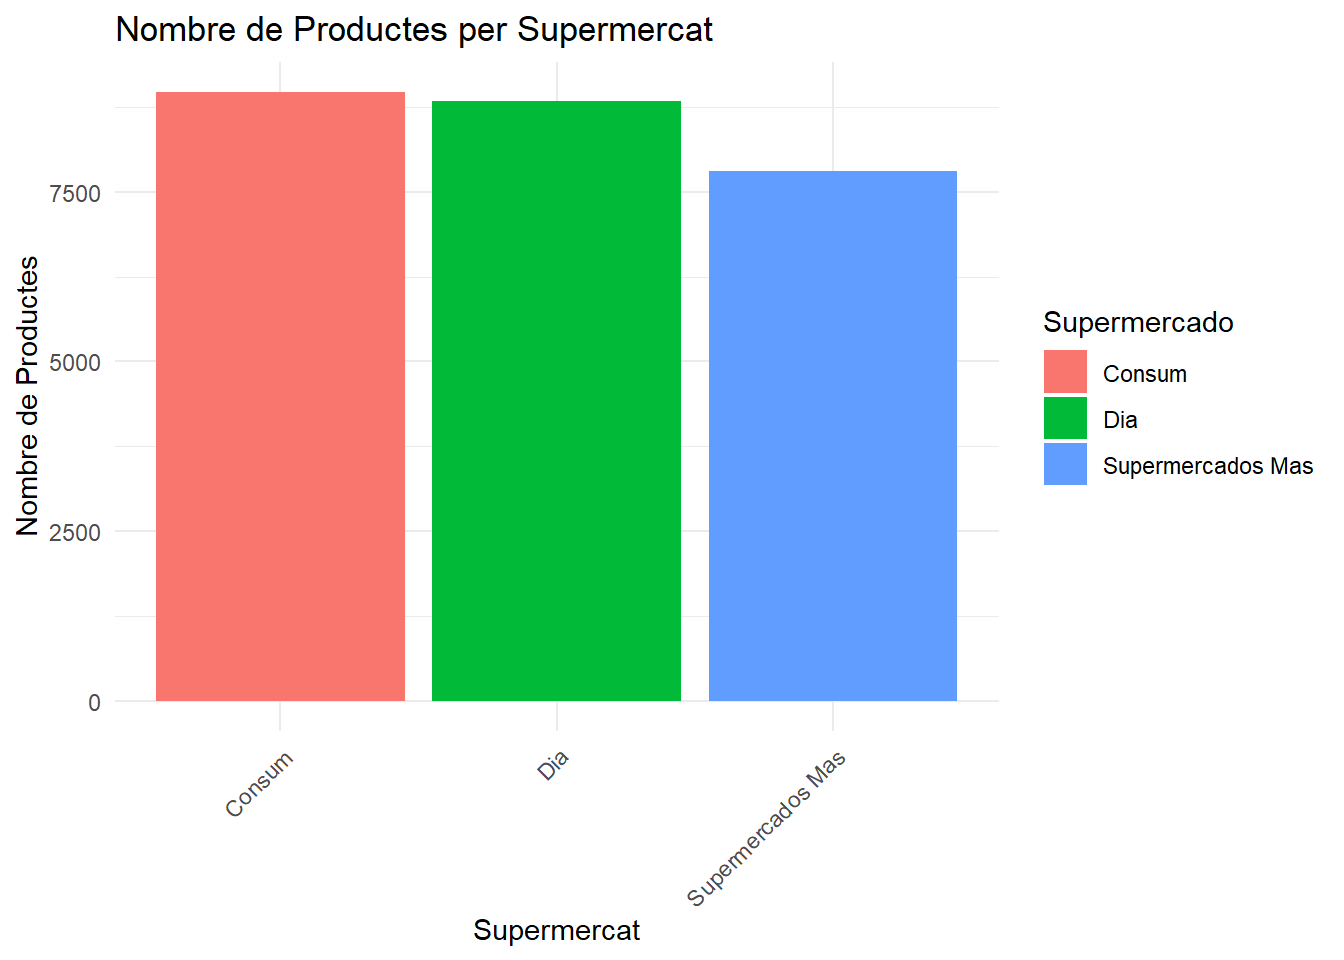
\includegraphics{Practica-2_files/figure-latex/unnamed-chunk-2-1.pdf}

\hypertarget{neteja-de-dades}{%
\section{Neteja de dades}\label{neteja-de-dades}}

\hypertarget{valors-faltants}{%
\subsection{Valors faltants}\label{valors-faltants}}

En primer lloc s'ha identificat aquells valors de les variables que
identifiquen valors faltants i s'ha trobat que a cada variable es
registre un cadena de caràters que descriu que hi ha un valor faltant.
Per exemple, a la variable \texttt{Nombre} s'han registrat els valors
faltants com \texttt{Nombre\ no\ disponible}, a \texttt{Marca}
\texttt{Marca\ no\ disponible}, i així successivament. Tots aquests
valors s'han substituït per \texttt{NA} per poder tractar les variables
correctament.

\hypertarget{tipus-de-dades}{%
\subsection{Tipus de dades}\label{tipus-de-dades}}

A continuació, s'han corregit totes les variables que contenien
caràcters especials i que no permeten tractar les variables així com és
degut. Per exemple, la variable \texttt{Precio} conté el signe € i per
tant no permet tractar la variable com un valor numèric. Llavors:

\begin{itemize}
\tightlist
\item
  \texttt{Nombre}: cadena de caràcters.
\item
  \texttt{Precio}: s'ha extret el signe €, els espais que hi podria
  haver i s'ha canviat les , dels decials per punts \texttt{.}.
  D'aquesta manera s'ha pogut transformar la variable a numèric.
\item
  \texttt{unidad}: s'ha convertit a factor i s'han unificat les
  categories que significaven el mateix. Per exemple: \texttt{1\ U},
  \texttt{Und.} i \texttt{UNIDAD} s'ha unificat a un sol nivell
  \texttt{UNIDAD}.
\item
  \texttt{precio\_unidad}: s'ha fet el mateix tractament que la variable
  \texttt{Precio} extraient signes i canviar les , dels decimals per
  punts. També s'ha trobat algún cas que s'utilitzava el \texttt{.} com
  a separadors del milers i també s'ha eliminat. Transformant posterior
  a valor numèric.
\item
  \texttt{Marca}: variable categòrica, per tant s'ha trasnformat a
  factor.
\item
  \texttt{Supermercat}: transformat a factor.
\item
  \texttt{Hora}: variable de tipus temps.
\item
  \texttt{Fecha}: variable de tipus data.
\item
  \texttt{Caregoría}: vairable categòrica, per tant, factor.
\item
  \texttt{Subcategoria}: conversió a factor.
\item
  \texttt{Estado}: conversió a factor.
\end{itemize}

Un cop transformades les dades correctament, s'estudien altres tipus de
valors que poden significar pèrdua de dades. Com per exemple, valors de
la variable \texttt{Precio} o \texttt{precio\_unitario} que tinguin
valors 0 o negatius. Entre aquests s'han trobat dos casos que tenen un
\texttt{precio\_unidad} igual a 0, degut al valor tant reduït que té
cada unitat d'aquests productes. Per evitar que aparegui el valor 0, es
calcularà manualment el valor real dividint el preu per les unitats de
cada article.

\hypertarget{tractament-de-valors-faltants}{%
\subsection{Tractament de valors
faltants}\label{tractament-de-valors-faltants}}

Un cop corregits els errors, hi ha que revistar i evaluar els valors
faltants \texttt{NA} de cada una de les variables.

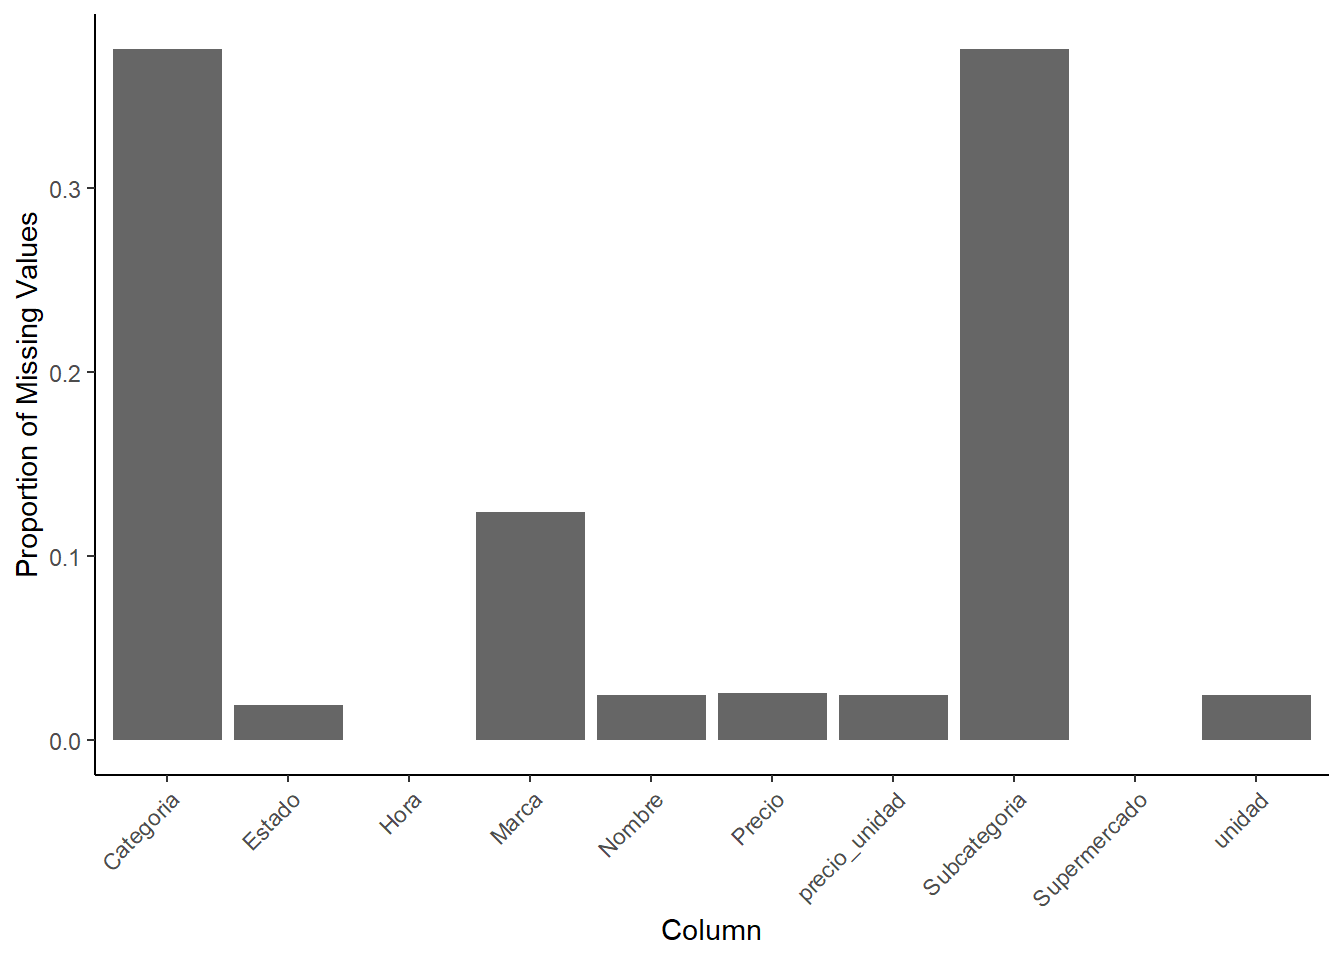
\includegraphics{Practica-2_files/figure-latex/faltantes-1.pdf}

Les variables \texttt{Marca}, \texttt{Categoría} y
\texttt{Subcategoría}, tenen una proporció de valors faltants elevats.
És evident que si s'esborressin tots els casos faltants d'aquestes
variables es perdrien molts casos i molta informació de valor per
l'anàlisi posterior. Per tant, s'ha cercat una alternativa per evitar
l'imputació de tots aquests valors. Aquesta alternativa consisteix en
utilitzar un algoritme per completar les seccions faltants a partir del
nom de cada producte. És a dir, a partir de les categories existents i
dels noms dels productes d'aquestes categories, es fa una estimació de
quina categoria pot ser la més adecuada per cada article li falta aquest
valor. Exactament, el que es fa és, per un producte sense categoria i
subcategoria, cercar els productes amb categoria i subcategoria
conegudes amb més paraules coincidents i assigna la categoria i
subcategoria més freqüents. Així i tot, hi ha productes que no s'ha
pogut classificar correctament, però tot i així s'ha reduït
considerablement els valors faltants.

Respecte a les altres variables es ronda un 2\% de valors faltants i
possiblament siguin els mateixos casos. Per tant, imputarem tots els
valors que no tenen un registre ni a la varaibles \texttt{Nombre},
\texttt{Precio}, \texttt{unidad} ni \texttt{precio\_unidad}, ja que no
aporten cap valor analític. Aquests casos signifiquen exactament 0.0244
de les files.

Per les dades que no tenen categoria ni subcategoria hem dit de
donar-los un valor fem una relació d'aquest registre per un nom semblant
en altres registres de cara a tenir un valor ``estimat'' d'aquestes dues
variables, graciés a l'ajuda dels altres registres.

\begin{Shaded}
\begin{Highlighting}[]
\CommentTok{\# Faltantes por supermercado}
\FunctionTok{table}\NormalTok{(productos\_actualizados}\SpecialCharTok{$}\NormalTok{Supermercado, }\FunctionTok{is.na}\NormalTok{(productos\_actualizados}\SpecialCharTok{$}\NormalTok{Categoria)) }\SpecialCharTok{\%\textgreater{}\%} \FunctionTok{prop.table}\NormalTok{(}\AttributeTok{margin =} \DecValTok{2}\NormalTok{)}
\end{Highlighting}
\end{Shaded}

\begin{verbatim}
##                    
##                         FALSE      TRUE
##   Consum            0.3576066 1.0000000
##   Dia               0.3292722 0.0000000
##   Supermercados Mas 0.3131212 0.0000000
\end{verbatim}

\begin{Shaded}
\begin{Highlighting}[]
\CommentTok{\# Faltantes por supermercado}
\FunctionTok{table}\NormalTok{(productos\_actualizados}\SpecialCharTok{$}\NormalTok{Supermercado, }\FunctionTok{is.na}\NormalTok{(productos\_actualizados}\SpecialCharTok{$}\NormalTok{Subcategoria)) }\SpecialCharTok{\%\textgreater{}\%} \FunctionTok{prop.table}\NormalTok{(}\AttributeTok{margin =} \DecValTok{2}\NormalTok{)}
\end{Highlighting}
\end{Shaded}

\begin{verbatim}
##                    
##                         FALSE      TRUE
##   Consum            0.3576066 1.0000000
##   Dia               0.3292722 0.0000000
##   Supermercados Mas 0.3131212 0.0000000
\end{verbatim}

\hypertarget{valors-extrems}{%
\subsection{Valors extrems}\label{valors-extrems}}

Per estudiar els valors extrems s'estudien els valors numèrics i
estudiarem els valors que poden distorsionar els estudis analítics.
Aquesta variable és: \texttt{Precio}.

El primer pas és estudiar la seva distribució, que es pot valorar tant
amb un diagrama de barres com amb un boxplot, que és on es veuen millor
els outliers.

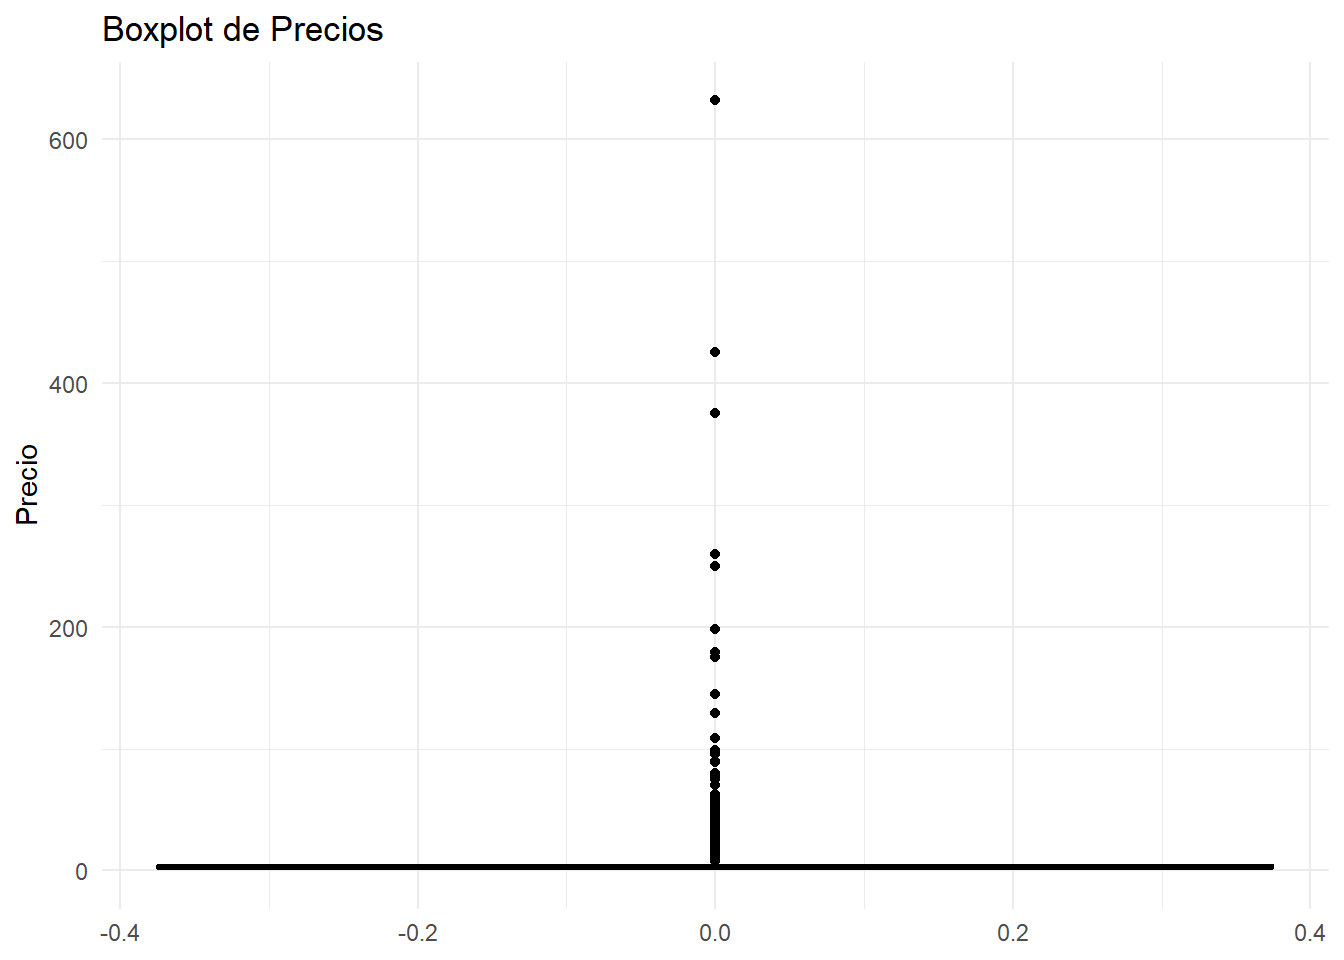
\includegraphics{Practica-2_files/figure-latex/unnamed-chunk-12-1.pdf}

Es pot veure com la variable \texttt{Precios} sí té valors extrems que
poden distorsionar les dades.

Un cop visualitzats els valors extrems, els podem detectar considerant
que un outlier son tots els punts que es troben a una distància del
primer o tercer quartil, més gran que 1.5 cops el rang interquantílic.
D'aquesta manera, al tenir identificats els valors extrems, podem
eliminar-los.

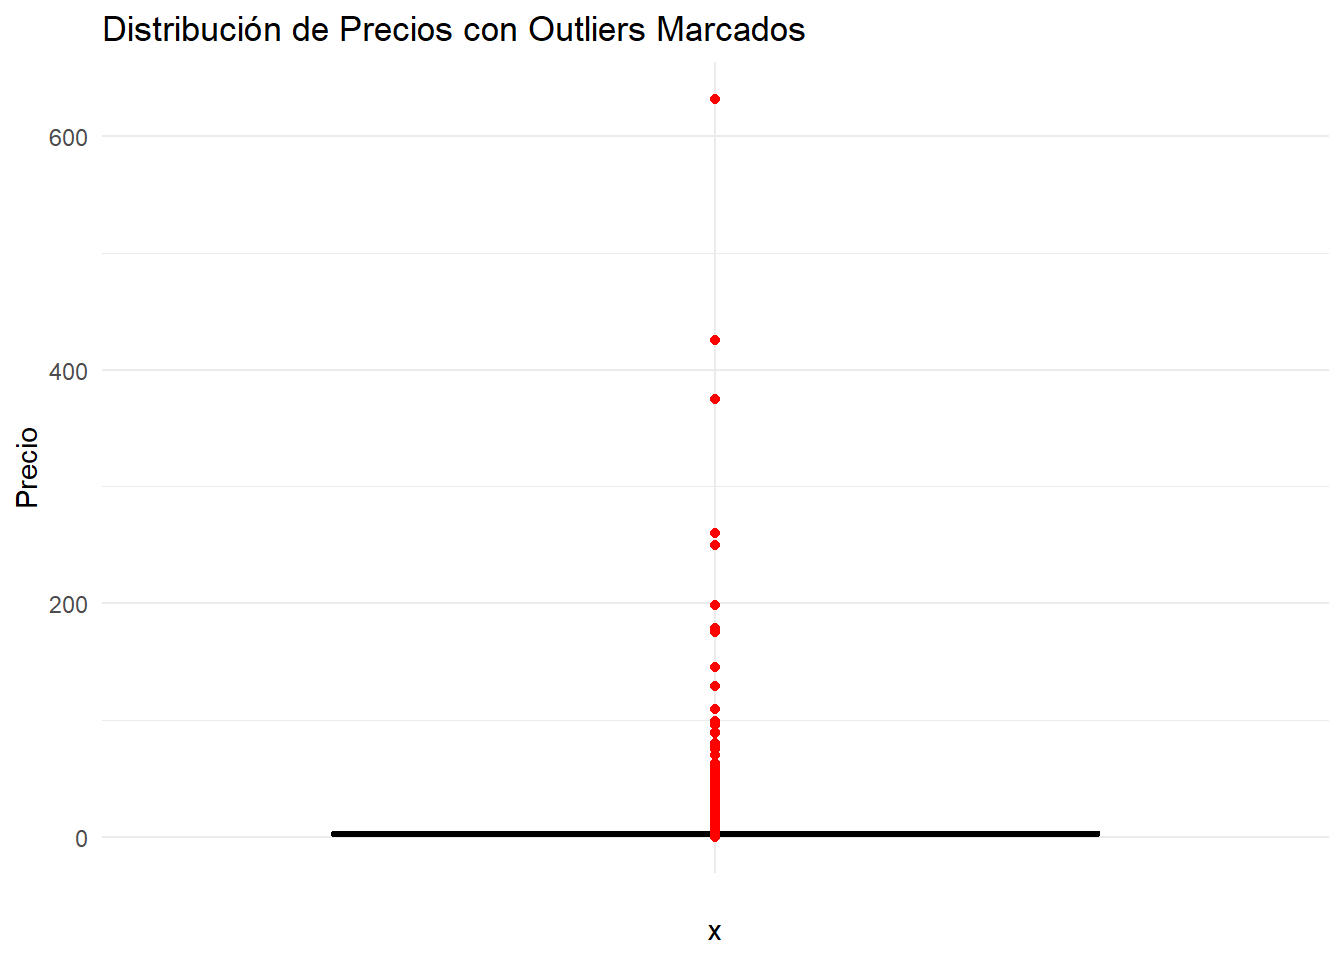
\includegraphics{Practica-2_files/figure-latex/unnamed-chunk-13-1.pdf}

En total s'han trobat 2603 del quals es reparteixen entre els
supermercats de la següent manera:

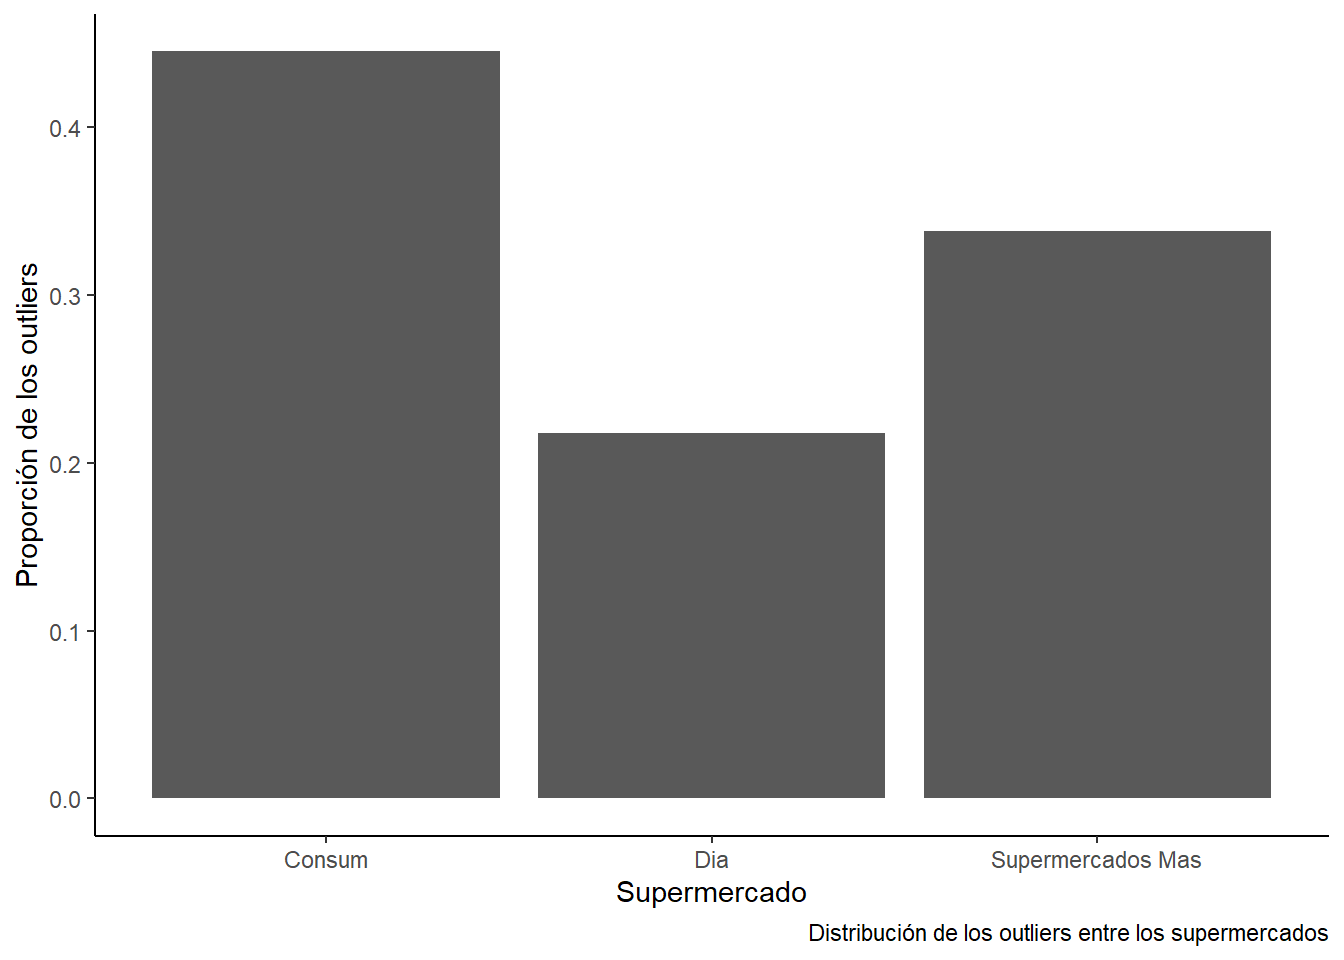
\includegraphics{Practica-2_files/figure-latex/unnamed-chunk-14-1.pdf}

Per tant, es por veure que quasi la meitat dels outliers trobats es
troben en el supermercat Consum, mentre que a Dia, és on hi ha menys
freqüència de outliers. Això no vol dir que Consum sigui el supermercat
més car, sinó que té més articles de preu elevat.

Tot i així, resvisant els valors extrems, considerem que no és necessari
corregir ni eliminar-los, ja que no es tracten d'errors d'entrada, sinó
que es tracta d'articles de més alta qualitat que tenen un preu alt,
però formen part de l'assortiment normal d'un supermercat. Així doncs,
formaràn part de les dades a analitzar.

\hypertarget{representaciuxf3-variables}{%
\subsection{Representació variables}\label{representaciuxf3-variables}}

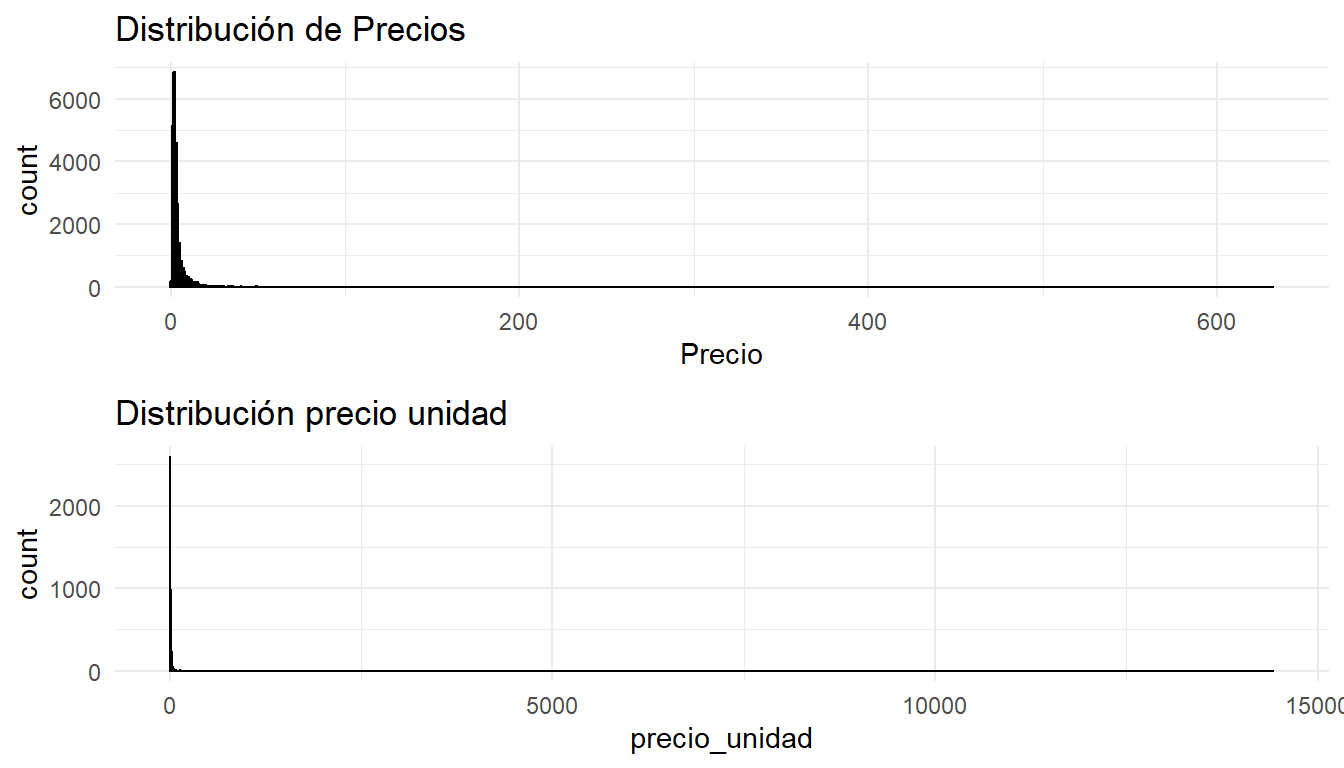
\includegraphics{Practica-2_files/figure-latex/unnamed-chunk-15-1.pdf}

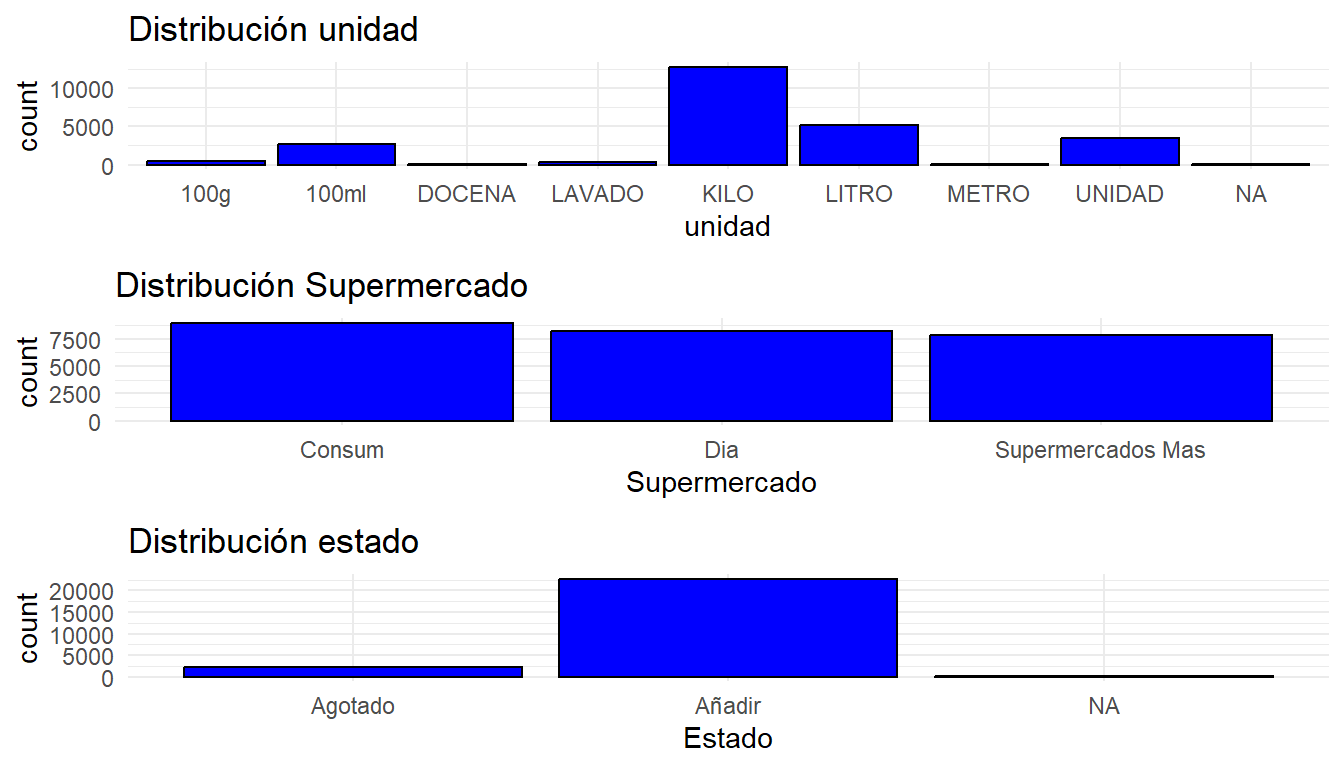
\includegraphics{Practica-2_files/figure-latex/unnamed-chunk-16-1.pdf}

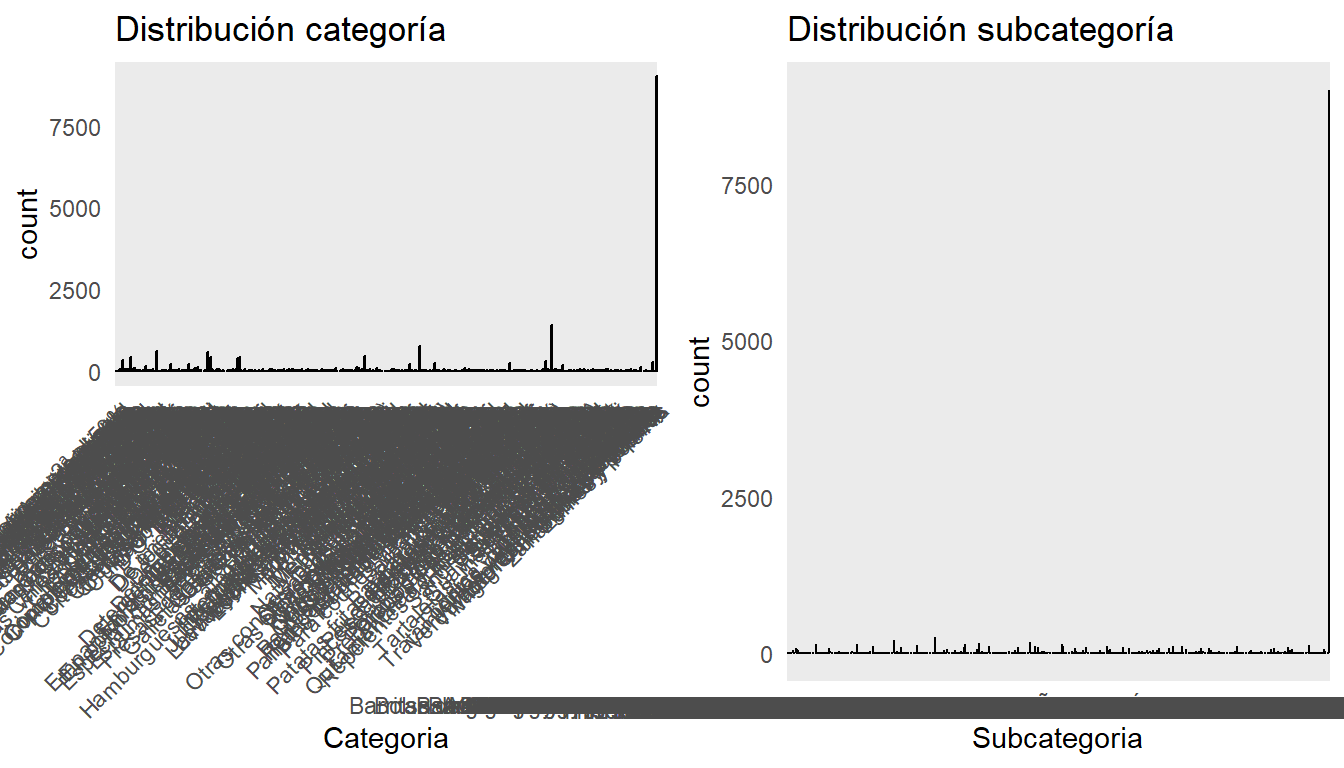
\includegraphics{Practica-2_files/figure-latex/unnamed-chunk-17-1.pdf}

\hypertarget{anuxe0lisi-de-les-dades}{%
\section{Anàlisi de les dades}\label{anuxe0lisi-de-les-dades}}

\hypertarget{models}{%
\subsection{Models}\label{models}}

\hypertarget{model-supervisat}{%
\subsubsection{Model supervisat}\label{model-supervisat}}

Basant-nos en les variables de unitat i supermercat, hem utilitzat un
model de regressió lineal per predir el preu del producte a la secció de
modelització supervisada. El model que hem definit cerca comprendre com
aquests elements afecten el preu final del producte. Per si de cas s'ha
eliminat la variable Preu els caràcters especials (€) i s'ha convertit
de text a numèric.

\begin{Shaded}
\begin{Highlighting}[]
\CommentTok{\# Asegurando que las variables están en formato adecuado}
\NormalTok{productos}\SpecialCharTok{$}\NormalTok{Precio }\OtherTok{\textless{}{-}} \FunctionTok{as.numeric}\NormalTok{(}\FunctionTok{gsub}\NormalTok{(}\StringTok{" €"}\NormalTok{, }\StringTok{""}\NormalTok{, }\FunctionTok{gsub}\NormalTok{(}\StringTok{","}\NormalTok{, }\StringTok{"."}\NormalTok{, productos}\SpecialCharTok{$}\NormalTok{Precio)))}

\CommentTok{\# Modelo de regresión lineal donde predecimos \textquotesingle{}Precio\textquotesingle{} basado en otras características:}
\NormalTok{modelo\_lineal }\OtherTok{\textless{}{-}} \FunctionTok{lm}\NormalTok{(Precio }\SpecialCharTok{\textasciitilde{}}\NormalTok{ unidad }\SpecialCharTok{+}\NormalTok{ Supermercado, }\AttributeTok{data =}\NormalTok{ productos\_actualizados)}
\FunctionTok{summary}\NormalTok{(modelo\_lineal)}
\end{Highlighting}
\end{Shaded}

\begin{verbatim}
## 
## Call:
## lm(formula = Precio ~ unidad + Supermercado, data = productos_actualizados)
## 
## Residuals:
##    Min     1Q Median     3Q    Max 
##  -6.08  -2.30  -1.16   0.28 628.07 
## 
## Coefficients:
##                               Estimate Std. Error t value Pr(>|t|)    
## (Intercept)                     2.2493     0.3941   5.707 1.16e-08 ***
## unidad100ml                     3.3384     0.4216   7.919 2.50e-15 ***
## unidadDOCENA                    0.3366     1.3330   0.253  0.80064    
## unidadLAVADO                    4.3098     0.5772   7.466 8.53e-14 ***
## unidadKILO                      1.3068     0.3974   3.288  0.00101 ** 
## unidadLITRO                     2.5454     0.4066   6.260 3.92e-10 ***
## unidadMETRO                     0.4068     1.6586   0.245  0.80627    
## unidadUNIDAD                    2.5403     0.4137   6.140 8.38e-10 ***
## SupermercadoDia                -0.8466     0.1236  -6.848 7.66e-12 ***
## SupermercadoSupermercados Mas   0.3721     0.1255   2.964  0.00304 ** 
## ---
## Signif. codes:  0 '***' 0.001 '**' 0.01 '*' 0.05 '.' 0.1 ' ' 1
## 
## Residual standard error: 8.059 on 24957 degrees of freedom
##   (34 observations deleted due to missingness)
## Multiple R-squared:  0.01406,    Adjusted R-squared:  0.01371 
## F-statistic: 39.56 on 9 and 24957 DF,  p-value: < 2.2e-16
\end{verbatim}

Els resultats obtinguts ens indiquen que diferents unitats i els
supermercats tenen un impacte estadísticament significatiu sobre el
preu. Per exemple, els coeficients per a les unitats com `100ml' i
`LAVADO' mostren increments notables en els preus, cosa que suggeriria
que aquestes unitats tendeixen a estar associades amb preus més alts.

Cal dir que , els supermercats també juguen un paper crucial en la
determinació dels preus. En particular, els productes del supermercat
Dia tendeixen a ser més barats en comparació amb la base. Aquest fet es
reflecteix en el coeficient negatiu per a Dia. En contrast, els
Supermercats Mas mostren un petit increment en els preus comparat amb el
supermercat de referència.

Podem veure que rl model té un R-quadrat ajustat relativament baix, cosa
que indica que les variables incloses expliquen només una petita part de
la variabilitat dels preus dels productes.

\hypertarget{model-no-supervisat}{%
\subsubsection{Model no supervisat}\label{model-no-supervisat}}

Hem desarrollat l'algorisme k-means per agrupar els productes en funció
dels seus preus i preus per unitat per a l'anàlisi no supervisada.
Primer per si de cas els preus s'han netejat i convertit en un format
numèric. Despues l'agrupació esta definida en tres grups.

\begin{Shaded}
\begin{Highlighting}[]
\NormalTok{productos}\SpecialCharTok{$}\NormalTok{Precio }\OtherTok{\textless{}{-}} \FunctionTok{as.numeric}\NormalTok{(}\FunctionTok{gsub}\NormalTok{(}\StringTok{" €"}\NormalTok{, }\StringTok{""}\NormalTok{, }\FunctionTok{gsub}\NormalTok{(}\StringTok{","}\NormalTok{, }\StringTok{"."}\NormalTok{, productos}\SpecialCharTok{$}\NormalTok{Precio)))}
\NormalTok{productos}\SpecialCharTok{$}\NormalTok{precio\_unidad }\OtherTok{\textless{}{-}} \FunctionTok{as.numeric}\NormalTok{(}\FunctionTok{gsub}\NormalTok{(}\StringTok{"€"}\NormalTok{, }\StringTok{""}\NormalTok{, }\FunctionTok{gsub}\NormalTok{(}\StringTok{","}\NormalTok{, }\StringTok{"."}\NormalTok{, productos}\SpecialCharTok{$}\NormalTok{precio\_unidad)))}

\NormalTok{productos }\OtherTok{\textless{}{-}}\NormalTok{ productos }\SpecialCharTok{\%\textgreater{}\%}
  \FunctionTok{filter}\NormalTok{(}\SpecialCharTok{!}\FunctionTok{is.na}\NormalTok{(Precio) }\SpecialCharTok{\&} \SpecialCharTok{!}\FunctionTok{is.na}\NormalTok{(precio\_unidad) }\SpecialCharTok{\&} 
         \SpecialCharTok{!}\FunctionTok{is.nan}\NormalTok{(Precio) }\SpecialCharTok{\&} \SpecialCharTok{!}\FunctionTok{is.nan}\NormalTok{(precio\_unidad) }\SpecialCharTok{\&}
\NormalTok{         Precio }\SpecialCharTok{!=} \ConstantTok{Inf} \SpecialCharTok{\&}\NormalTok{ Precio }\SpecialCharTok{!=} \SpecialCharTok{{-}}\ConstantTok{Inf} \SpecialCharTok{\&} 
\NormalTok{         precio\_unidad }\SpecialCharTok{!=} \ConstantTok{Inf} \SpecialCharTok{\&}\NormalTok{ precio\_unidad }\SpecialCharTok{!=} \SpecialCharTok{{-}}\ConstantTok{Inf}\NormalTok{)}

\FunctionTok{set.seed}\NormalTok{(}\DecValTok{123}\NormalTok{)}

\CommentTok{\# Ejecutar k{-}means con 3 centros}
\NormalTok{kmeans\_resultado }\OtherTok{\textless{}{-}} \FunctionTok{kmeans}\NormalTok{(productos[, }\FunctionTok{c}\NormalTok{(}\StringTok{"Precio"}\NormalTok{, }\StringTok{"precio\_unidad"}\NormalTok{)], }\AttributeTok{centers =} \DecValTok{3}\NormalTok{)}

\CommentTok{\# Agregar los clusters al dataframe para análisis posterior}
\NormalTok{productos}\SpecialCharTok{$}\NormalTok{Cluster }\OtherTok{\textless{}{-}} \FunctionTok{as.factor}\NormalTok{(kmeans\_resultado}\SpecialCharTok{$}\NormalTok{cluster)}

\CommentTok{\# Visualizar los resultados de k{-}means}

\FunctionTok{ggplot}\NormalTok{(productos, }\FunctionTok{aes}\NormalTok{(}\AttributeTok{x =}\NormalTok{ Precio, }\AttributeTok{y =}\NormalTok{ precio\_unidad, }\AttributeTok{color =}\NormalTok{ Cluster)) }\SpecialCharTok{+}
  \FunctionTok{geom\_point}\NormalTok{(}\AttributeTok{alpha =} \FloatTok{0.5}\NormalTok{) }\SpecialCharTok{+}
  \FunctionTok{labs}\NormalTok{(}\AttributeTok{title =} \StringTok{"Clustering de Productes por Preu y Preu por Unidad"}\NormalTok{) }\SpecialCharTok{+}
  \FunctionTok{theme\_minimal}\NormalTok{()}
\end{Highlighting}
\end{Shaded}

\includegraphics{Practica-2_files/figure-latex/unnamed-chunk-19-1.pdf}

Com odem veure en es el gràfic els productes han estat dividits en tres
clústers diferents, cada un representat per un color diferent:

\begin{itemize}
\item
  Clúster 1 (Color vermell): Aquest grup conté productes amb preus més
  baixos i preus per unitat relativament baixos. Podem dir que son els
  productes bàsics o de consum diari més assequibles.
\item
  Clúster 2 (Color blau): Els productes d'aquest grup semblen tenir
  preus més elevats, però encara amb preus per unitat baixos, podem dir
  que podria incloure articles venuts en major quantitat o en format a
  granel.
\item
  Clúster 3 (Color verd): Aquí veiem pocs productes que tenen preus per
  unitat significativament alts. Podrien ser productes especialitzats o
  de luxe.
\end{itemize}

\hypertarget{prueba-de-contraste-de-hipuxf3tesis}{%
\subsection{Prueba de Contraste de
Hipótesis}\label{prueba-de-contraste-de-hipuxf3tesis}}

Hem dut a terme una prova de contrast d'hipòtesis, enfocant-te
específicament en els que contenien ``Jamon'' en nom seu. El procés
inclou la neteja de dades, la conversió del preu de text a números i la
creació d'una variable per determinar si el producte conté ``Jamon'' en
el nom.

\begin{Shaded}
\begin{Highlighting}[]
\NormalTok{productos}\SpecialCharTok{$}\NormalTok{Precio }\OtherTok{\textless{}{-}} \FunctionTok{as.numeric}\NormalTok{(}\FunctionTok{gsub}\NormalTok{(}\StringTok{" €"}\NormalTok{, }\StringTok{""}\NormalTok{, }\FunctionTok{gsub}\NormalTok{(}\StringTok{","}\NormalTok{, }\StringTok{"."}\NormalTok{, productos}\SpecialCharTok{$}\NormalTok{Precio)))  }\CommentTok{\# Limpieza de datos}

\CommentTok{\# Agregamos una nueva columna para identificar si el nombre del producto contiene \textquotesingle{}Jamon\textquotesingle{}}
\NormalTok{productos }\OtherTok{\textless{}{-}}\NormalTok{ productos }\SpecialCharTok{\%\textgreater{}\%}
  \FunctionTok{mutate}\NormalTok{(}\AttributeTok{contiene\_Jamon =} \FunctionTok{ifelse}\NormalTok{(}\FunctionTok{grepl}\NormalTok{(}\StringTok{"Jamon"}\NormalTok{, Nombre, }\AttributeTok{ignore.case =} \ConstantTok{TRUE}\NormalTok{), }\StringTok{"Con Jamon"}\NormalTok{, }\StringTok{"Sin Jamon"}\NormalTok{))}

\CommentTok{\# Calculamos el precio medio general excluyendo NA}
\NormalTok{precio\_medio\_general }\OtherTok{\textless{}{-}} \FunctionTok{mean}\NormalTok{(productos}\SpecialCharTok{$}\NormalTok{Precio, }\AttributeTok{na.rm =} \ConstantTok{TRUE}\NormalTok{)}

\CommentTok{\# Subconjunto de productos que contienen \textquotesingle{}Jamon\textquotesingle{} en el nombre}
\NormalTok{productos\_con\_Jamon }\OtherTok{\textless{}{-}}\NormalTok{ productos }\SpecialCharTok{\%\textgreater{}\%}
  \FunctionTok{filter}\NormalTok{(contiene\_Jamon }\SpecialCharTok{==} \StringTok{"Con Jamon"}\NormalTok{) }\SpecialCharTok{\%\textgreater{}\%}
  \FunctionTok{pull}\NormalTok{(Precio)}

\CommentTok{\# Prueba de normalidad}
\NormalTok{shapiro\_test\_Jamon }\OtherTok{\textless{}{-}} \FunctionTok{shapiro.test}\NormalTok{(productos\_con\_Jamon)}
\FunctionTok{print}\NormalTok{(shapiro\_test\_Jamon)}
\end{Highlighting}
\end{Shaded}

\begin{verbatim}
## 
##  Shapiro-Wilk normality test
## 
## data:  productos_con_Jamon
## W = 0.35624, p-value < 2.2e-16
\end{verbatim}

\begin{Shaded}
\begin{Highlighting}[]
\CommentTok{\# Dependiendo de la normalidad, realizar t{-}test o Wilcoxon test}
\ControlFlowTok{if}\NormalTok{ (shapiro\_test\_Jamon}\SpecialCharTok{$}\NormalTok{p.value }\SpecialCharTok{\textgreater{}} \FloatTok{0.05}\NormalTok{) \{}
\NormalTok{  t\_test\_result }\OtherTok{\textless{}{-}} \FunctionTok{t.test}\NormalTok{(productos\_con\_Jamon, }\AttributeTok{mu =}\NormalTok{ precio\_medio\_general)}
  \FunctionTok{print}\NormalTok{(t\_test\_result)}
\NormalTok{\} }\ControlFlowTok{else}\NormalTok{ \{}
  \FunctionTok{print}\NormalTok{(}\StringTok{"Distribución no normal, aplicando prueba no paramétrica."}\NormalTok{)}
\NormalTok{  wilcox\_test\_result }\OtherTok{\textless{}{-}} \FunctionTok{wilcox.test}\NormalTok{(productos\_con\_Jamon, }\AttributeTok{mu =}\NormalTok{ precio\_medio\_general, }\AttributeTok{alternative =} \StringTok{"greater"}\NormalTok{)}
  \FunctionTok{print}\NormalTok{(wilcox\_test\_result)}
\NormalTok{\}}
\end{Highlighting}
\end{Shaded}

\begin{verbatim}
## [1] "Distribución no normal, aplicando prueba no paramétrica."
## 
##  Wilcoxon signed rank test with continuity correction
## 
## data:  productos_con_Jamon
## V = 844, p-value = 0.9989
## alternative hypothesis: true location is greater than 4.055195
\end{verbatim}

Podem veure a partir dels resultats de la prova de Shapiro-Wilk, s'ha
determinat que la distribució dels preus dels productes que contenen
``Jamon'' no és normal, ja que el p-valor és significativament menor que
0.05. Per això ens portat a l'aplicació d'una prova no paramètrica,
específicament el test de Wilcoxon, en comptes d'un t-test que requereix
normalitat en les dades on el p-valor de 0.9989, suggerint que no hi ha
evidència estadísticament significativa per rebutjar la hipòtesi nul·la
que el preu mitjà dels productes que contenen ``Jamon'' és major que el
preu mitjà general dels productes.

\hypertarget{resoluciuxf3-del-problema}{%
\section{Resolució del problema:}\label{resoluciuxf3-del-problema}}

Podem dir que hem arribat a diverses conclusions importants a partir de
l'anàlisi i els resultats de la investigació del conjunt de dades dels
preus dels supermercats que ens permeten abordar els primers problemes:

Conclusions:

\begin{itemize}
\item
  Variabilitat de preus entre cadenes: Podem veure que segons la cadena
  de supermercats, hi ha diferències significatives en el preu d'un
  producte. En particular dir que, els preus del supermercat Dia han
  estat generalment més baixos que els de Consum i Supermercats Mas.
\item
  Impacte de les unitats de mesura en el preu: Podem veure que segons el
  model de regressió lineal, les unitats de mesura com a litres i
  quilograms tenen un impacte significatiu en el preu d'un producte. I
  podem dir que els preus dels productes que es mesuren per unitats
  grans solen ser més alts, cosa que indica una estratègia de preus
  basada en el volum de venda.
\item
  Segmentació de productes per preu: Podem veure ham la utilització de
  l'algorisme k-means per agrupar productes, que s'han identificat grups
  clars basats en el preu i el preu per unitat. Aquí es mostra la
  diversitat de l'oferta de les cadenes de supermercats i pot ajudar els
  clients a identificar quins supermercats ofereixen els millors preus
  per a productes específics o en grans quantitats.
\item
  Normalitat i distribució de preus: I com punt final podem véreu que
  les proves de contrast d'hipòtesis han demostrat que la distribució de
  preus dels articles amb Jamon no segueix una distribució normal, cosa
  que ha requerit l'ús de proves no paramètriques. Aquestes proves han
  demostrat que no hi ha diferències significatives en el preu mitjà
  dels productes amb ``Jamon'' en comparació del preu mitjà general.
\item
  Per concloure dir que els resultats de l'anàlisi demostren la utilitat
  dels models estadístics i les tècniques de mineria de dades en la
  comparació dels preus dels supermercats, proporcionant solucions
  clares i útils al problema plantejat.
\end{itemize}

\hypertarget{codi}{%
\section{Codi}\label{codi}}

El codi font desenvolupat per a la neteja, anàlisi i representació de
dades ha estat principalment desenvolupat en R. Ja escollit per la seva
flexibilitat, poder estadístic i la disponibilitat d'una àmplia
biblioteca de paquets específics per a la manipulació de dades i
visualització gràfica.

En elcodi en R hem utilitzat diverses llibreries crucials per al
processament i anàlisi de dades com dplyr per a la manipulació de dades,
ggplot2 per a la visualització, i readr per a la càrrega eficient de
dades. Dir que per la neteja de dades, s'han implementat rutines
específiques que tracten amb valors faltants, correcció de formats i la
normalització de les cadenes de text. Aquestes tasques són necessàries
per assegurar la qualitat i la consistència dels conjunts de dades amb
els quals s'analitzen.

Podem veure també que en el codi per a l'anàlisi de les dades hem
desenvolupat models estadístics com regressions lineals i algoritmes de
clustering (k-means). Méstard hem fet les visualitzacions dels resultats
d'anàlisis en difuntes tipus de gràfics.

Dir que el codi font està disponible de manera pública en el següent
enllaç del repositori GitHub, que conté tots els scripts utilitzats així
com documentació addicional sobre l'estructura i l'ús dels codis:

\url{https://github.com/cromeroUOC/Analysis-Web-Scraping-Supermarket}

\hypertarget{referuxe8ncies}{%
\section{Referències}\label{referuxe8ncies}}

\begin{itemize}
\item
  RPubs - Clase 6 - Limpieza de datos. (n.d.).
  \url{https://rpubs.com/camilamila/limpieza}
\item
  kmeans function - RDocumentation. (n.d.).
  \url{https://www.rdocumentation.org/packages/stats/versions/3.6.2/topics/kmeans}
\item
  RPubs - Introducción a los Modelos de Agrupamiento en R. (n.d.).
  \url{https://rpubs.com/rdelgado/399475}
\item
  RPubs - Regresión lineal simple. (n.d.).
  \url{https://rpubs.com/joser/RegresionSimple}
\item
  RPubs - Market Basket Analysis on Groceries Data. (n.d.).
  \url{https://rpubs.com/Handedemirci/1011420}
\end{itemize}

\hypertarget{taula-de-contribucions}{%
\section{Taula de Contribucions}\label{taula-de-contribucions}}

\begin{longtable}[]{@{}ll@{}}
\caption{Resum de Contribucions}\tabularnewline
\toprule\noalign{}
Contribucions & Signatura \\
\midrule\noalign{}
\endfirsthead
\toprule\noalign{}
Contribucions & Signatura \\
\midrule\noalign{}
\endhead
\bottomrule\noalign{}
\endlastfoot
Investigació prèvia & CRM, ESA \\
Redacció de les respostes & CRM, ESA \\
Desenvolupament del codi & CRM, ESA \\
Participació al vídeo & CRM, ESA \\
\end{longtable}

CRM: Carlos Romero Matarin ESA: Enric Sintes Arguimbau

\end{document}
